\documentclass[a4paper,10pt]{article}

\usepackage[margin=2cm]{geometry}
\usepackage{graphicx}
\usepackage{hyperref}
\usepackage[all]{hypcap}
\usepackage{tabu}
\usepackage[title,titletoc,toc]{appendix}
\usepackage[english]{babel}
\usepackage{float}
\usepackage{fancyhdr}
\usepackage{microtype}
\graphicspath{ {images/} }

\setlength{\headheight}{15.2pt}
\pagestyle{fancy}
\lhead{Bellisimo}
\chead{}
\rhead{\bfseries Software Requirements Specification}
\lfoot{COS731 Software Engineering}
\rfoot{Page \thepage}
\cfoot{}
\renewcommand{\headrulewidth}{0.4pt}
\renewcommand{\footrulewidth}{0.4pt}

\setlength{\parindent}{0pt}
\setlength{\parskip}{1ex plus 0.5ex minus 0.2ex}

\frenchspacing

\title{
\includegraphics[width=12cm]{Eeufeeslogo.jpg} \\       
      \bfseries Bellisimo \\
       \vspace{1.0cm}
       Software Requirements Specification \\ 
       \vspace{0.5cm}
       }

\date{\today} 
\author{Elizabeth (EF) Bode			14310156}

\begin{document}
\maketitle
\thispagestyle{empty}

\newpage
\pagenumbering{roman}
\thispagestyle{empty}
\tableofcontents
\clearpage

\newpage
\pagenumbering{arabic}

\section{Business Requirements}
\subsection{Background}
Bellisimo is a company aimed at providing an online platform for customers to browse clothing as well as food catalogues provided by the business located in Hatfield. Information about specials and promotions will be published on the online platform.

\subsection{Vision}
The core of the system will be catalogues of items and their prices. Since Bellisimo is involved in clothing and food, the catalogues will have to ensure that these lines are well maintained. Sales and specials in each line will have to be accounted for and managed.

\subsection{Scope}
Bellisimo will be a web-based application that provides the functionalities of an online catalogue for food and clothing. The application will be accessible from anywhere using a specified URL. The goal of the system is to provide Bellisimo’s customers with the latest information on their food and clothing products and the specials associated with them.

\subsection{System Functions}
\begin{itemize}
	\item An admin interface to allow for adding, removing and updating product items and specials
	\item An anonymous user interface to allow for browsing, searching and filtering products and viewing the details of a product and the specials that are running
	\item An admin user should be able to login, logout and manage their profile
\end{itemize}

\subsection{Assumptions}
\begin{itemize}
	\item An admin user has to be preloaded onto the system, the system doesn’t cater for adding admin users to it
\end{itemize}

\subsection{Constraints}
\begin{itemize}
	\item The system must be implemented using the technologies stated in the provided specification
	\item Only open source software should be used for the system
	\item The system must be complete by the 6th September
\end{itemize}

\subsection{Methodology}
This system will be implemented using the Agile methodology as this methodology allows flexibility in regards to changing requirements. Scrum will also be incorporated into the Agile methodology as it provides a suitable framework for project management. Milestones and issues will be set up on Github to keep track of tasks that are outstanding. These milestones and issues will be linked to waffle.io in order to provide an interactive interface showing completed tasks and outstanding tasks. This will also be linked to burndown.io as it provides a burndown chart for your project showing overall progress according to time constraints.

\section{System Requirements and Design}
\subsection {Architectural Design}
\subsubsection{Overview}
The web application will consist of two subsystems that communicate via HTTP using REST Framework. The Java/Spring Boot application will be known as the "backend" application. The HTML5/Angular2 application will be known as the "frontend" application. The backend application is expected to communicate with the database and use Hibernate which can be imported into Maven, a dependency management tool whereas the frontend application will be hosted in the browser and NodeJS is expected to manage packages required for the application to run successfully.

\subsubsection{Micro-services Architecture}
The micro services implementation will consist on n spring boot applications where n = no. of modules or components in the system. These applications will be integrated by using spring cloud and Netflix OSS Zuul Integration. The integration server will be regarded as one component of the n components to be implemented.
\begin{figure}[H]
	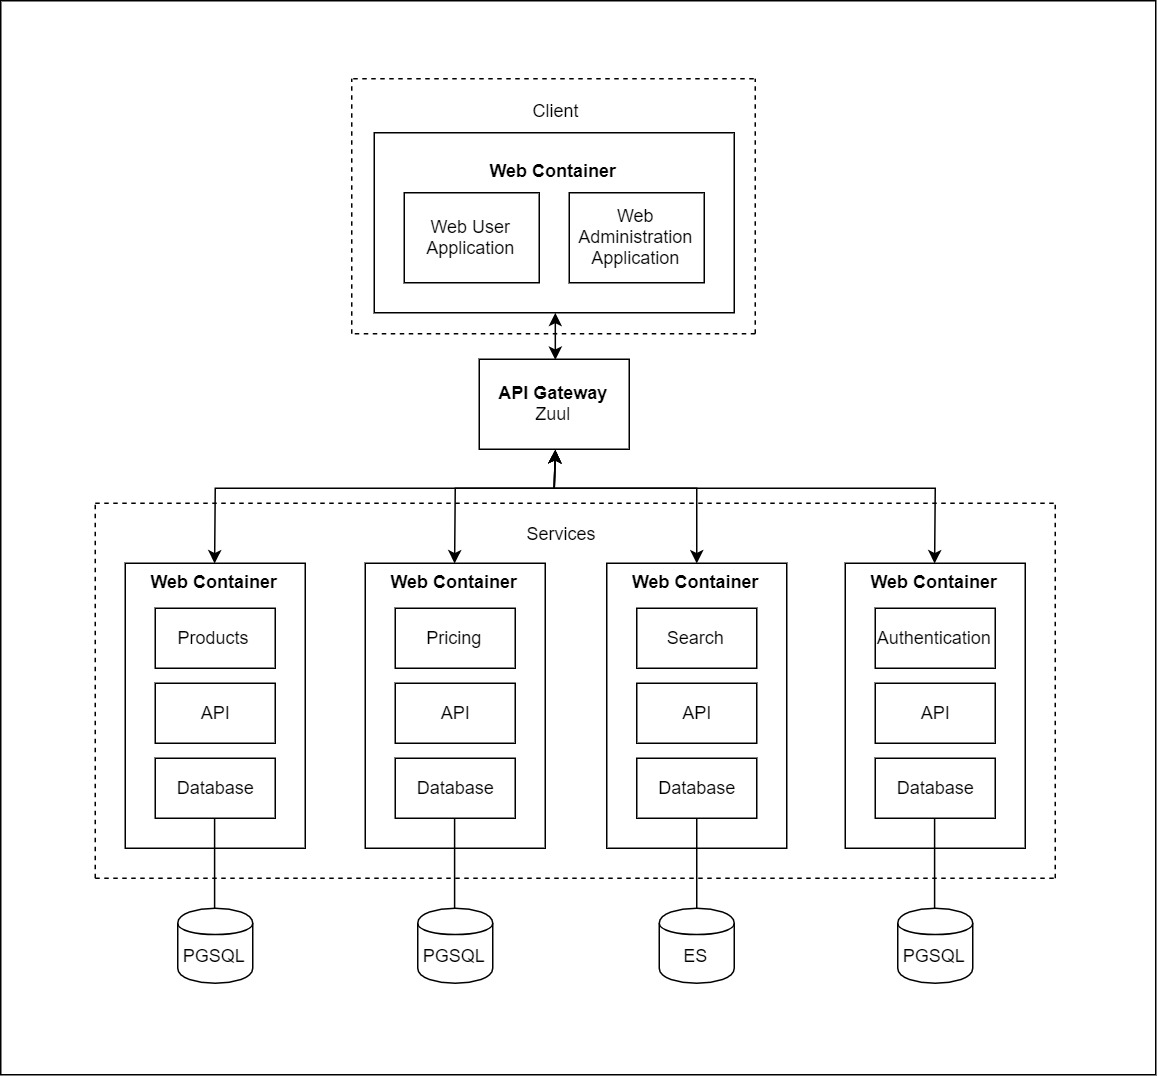
\includegraphics[scale=0.5]{component_diagram}
	\caption{System components diagram}
\end{figure}

\subsubsection{Non-Functional Requirements}
\begin{itemize}
	\item  \textbf{Performance} \\\\
	System performance can be defined as the amount of work the system can perform in a measured time interval. The time interval is normally measured in seconds, where the amount of work can be defined as the throughput, latency or data transmission time.\\\\
	 \underline{Requirements:}
	 \begin{itemize}
		\item Function calls must be timed and benchmarked and this data should be logged
		\item Network responses should be cached on server side to lighten the load on database as well as decreasing the round trip time of request - response
		\item The system should never hang because of poor system performance, it should only be a result of a poor network connection
	\end{itemize}
	\item  \textbf{Integrability} \\\\
	Integrability refers to a system’s ability to seamlessly integrate new modules into the existing system regardless of the varying technologies they were implemented in.\\\\
	 \underline{Requirements:}
	 \begin{itemize}
		\item The system should allow technology neutral importing and exporting of data
		\item The back-end system should integrate with a desktop web client
		\item The system should be able to integrate with different back-end authentication services
		\item Modules should be able to be swapped in and out regardless of the technologies they are implemented in
	\end{itemize}
	\item  \textbf{Maintainability} \\\\
	The system is to be designed in such a way that it is easily updated, modified or extended by the client in the future. In order to achieve these requirements, design patterns and best practices will be used to ensure uniformity and modularity across the system.\\\\
	 \underline{Requirements:}
	 \begin{itemize}
		\item All code should be documented in the applicable language documentation framework, such as JavaDocs for a Java based system, DOxygen for a C/C++ based system, etc. 
		\item A specified coding style should be adhered to so as to enforce readable code that is consistent and easier to maintain
		\item System should be separated in distinct, concise and independent modules relating to separate concerns, to allow for easier maintenance
	\end{itemize}
	\item  \textbf{Scalability} \\\\
	Scalability refers to the application in question’s ability to handle an above normal workload for extended time periods and the mechanisms employed to facilitate this.\\\\
	 \underline{Requirements:}
	 \begin{itemize}
		\item The system should be able to handle increased workloads towards the end of the month when people are paid
		\item The system should be able to facilitate 100 concurrent user sessions at any time
	\end{itemize}
	\item  \textbf{Reliability} \\\\
	System reliability refers to the probability of the system performing an operation to a satisfactory standard at or for a specified time in a specified environment.\\\\
	 \underline{Requirements:}
	 \begin{itemize}
		\item The system should never go down as it could potentially cause Bellisimo to lose several customers
		\item The system should have the ability to swap out modules without causing system downtime
	\end{itemize}
	\item  \textbf{Security} \\\\
	Security comprises of data security authentication and authroization. Authentication refers the system’s ability to identify a user to be who they are. Authorization refers to the system’s ability to provide the user in question with access to only the system functions that they have the authority to perform. Data security 			refers to data only being accessible through authorized channels.\\\\
	 \underline{Requirements:}
	 \begin{itemize}
		\item System should be resistant to SQL injections
		\item Password hosting with a unique salt for each user should be used
		\item A key derivation function should be used with passwords
		\item Database access must require authentication
	\end{itemize}
	\item  \textbf{Accessibility} \\\\
	System accessibility refers to the system being accessible to whomever requires it when they require it.\\\\
	 \underline{Requirements:}
	 \begin{itemize}
		\item The system should have a web interface that’s hosted on a server so customers can access it wherever whenever
		\item The system won’t take into account any individual with any type of disability hindering their interaction with a web-based application
	\end{itemize}
	\item  \textbf{Flexibility} \\\\
	Flexibility refers to the system’s ability to continue to function regardless of internal swapping of components. Furthermore, it refers to the system’s ability to be able to adapt to changing constraints.\\\\
	 \underline{Requirements:}
	 \begin{itemize}
		\item The system should be decoupled from the database technology it uses and allow the client to select and change the database it uses in future
		\item Authentication mechanisms used should be decoupled from the system, allowing them to be interchangeable
		\item Modules should be decoupled from one another, allowing the system to be extensible without a break in service which is achieved by integrating new modules and swapping out existing ones
	\end{itemize}
\end{itemize}

\subsubsection{Architectural Patterns}
\begin{itemize}
	\item \textbf {Authentication Enforcer Pattern} \\\\
	The authentication enforcer pattern provides centralized management for authentication, to verify the identity of users and encapsulate the details of authentication. This pattern enforces that security checks are separated from business logic, ensuring cleaner and more robust code, promoting easier maintenance. Since 	authentication is centralized, this pattern also allows changes to be easily implemented in regards to the authentication procedure, allowing one to substitute authentication procedures without having to recode the entire system. \\\\
	\underline{Reasons for selecting this pattern:}
	\begin{itemize}
		\item This pattern promotes reliability because authentication is centralized allowing system modules to be swapped in and out or upgraded without affecting the system’s reliability, as long as the authentication mechanism provides the same service to the system
		\item This pattern promotes flexibility as it allows for integration of varying technologies, giving the developer freedom in regards to the technologies they want to use for authentication
		\item This pattern promotes maintainability and integrability as authentication mechanisms are decoupled and interchangeable and can be used wherever the system requires authentication by simply plugging in the appropriate module\\
	\end{itemize}
	
	\item \textbf {Client-Server Architectural Pattern} \\\\
	A network technology in which each computer connected on the network is either a server or client is called a client server architecture. An interface is provided by the client to allow a user to request services from the server and to display the results the server returns. 
	\begin{enumerate}
		\item Servers: are powerful computers which are used to process the client requests
		\item Client: is simply a computer connected to the network which is used to send requests for resources to the server\\
	\end{enumerate}
	\underline{Reasons for selecting this pattern:}
	\begin{itemize}
		\item This pattern promotes maintainability and flexibility  as it allows decoupling of business logic and human adapter modules
		\item It enables system usability by not requiring users to incur large downloads to make use of the system
		\item The pattern promotes maintainability and reliability, since developers are able to upgrade and update individual system modules without affecting any other modules\\
	\end{itemize}
	\item \textbf {Layered Architectural Pattern} \\\\
	A design pattern in which software is divided up into individual layers by functionality. The layers interact with one another via requests and responses, and there are typically four of these layers:
	\begin{enumerate}
		\item Presentation/view: The user interface that the user interacts with, such as a desktop client
		\item Application/controller: The service API that the presentation layer interacts with in order to perform system functions
		\item Business logic: The functions that get called by the service API, to interact with system data
		\item Data access: The layer that provides data access to the business logic layer\\
	\end{enumerate}
	\underline{Reasons for selecting this pattern:}
	\begin{itemize}
		\item This pattern promotes reliability, flexibility, integrability and maintainability as it enables trivial swapping of groups of modules
		\item The pattern promotes maintainability as it allows decoupling of the database and authentication modules from the rest of the system\\
	\end{itemize}
	\item \textbf {Representational State Transfer (REST) Architectural Pattern} \\\\
	REST is an architectural pattern for designing networked applications. The idea is instead of using complex mechanisms such as SOAP, CORBA or RPC to connect between machines or to make calls between machines, HTTP is used. A REST service is: 
	\begin{enumerate}
		\item Language-independent (C\# can communicate to Java, etc.)
		\item Can be used with firewalls
		\item Platform-independent (MAC, Windows, UNIX)
		\item Standards-based (runs on top of HTTP) \\
	\end{enumerate}
	\underline{Reasons for selecting this pattern:}
	\begin{itemize}
		\item It promotes flexibility since it allows platform independent communication between business logic and human adapter modules
		\item It promotes maintainability as it is language independent and allows for easy migration of services to different technologies while keeping communication methods well defined
		\item It satisfies the performance requirement as REST network responses can be cached\\
	\end{itemize}
	\item \textbf {Services Orientated Architecture/ Micro-services Architecture} \\\\
	An architectural pattern in software design in which system use cases are divided into one or more service operations, and these service operations are then implemented, either individually or combined with other service operations, by a reusable SOA service. The SOA architecture itself comprises five layers: 
	\begin{enumerate}
		\item Consumer interface: The GUI for end users accessing application services 
		\item Business process: The representation of system use cases 
		\item Services: The consolidated inventory of all available services
		\item Service components: The reusable components used to build the services, such as functional libraries
		\item Operational system: Contains data repository, technological platforms, etc. \\
	\end{enumerate}
	This architectural pattern provides an aggregated collection of services which implement the use cases of the system. The user or developer themselves can choose which of these available services to call on.\\\\
	\underline{Reasons for selecting this pattern:}
	\begin{itemize}
		\item This pattern promotes system reliability and scalability as it focuses on decoupling service objects so they can be distributed on different machines and can be implemented using varying technologies
		\item This pattern promotes system flexibility as the decoupling of service objects allows for interchangeable service providers, ensuring the system is never restricted by its service providers if conditions change and require upgrades or updates
		\item This pattern satisfies all the same quality requirements as the layered architecture pattern
	\end{itemize}
\end{itemize}



\newpage
\clearpage



\end{document}